\chapter{Referencial Teórico}
\label{ch:referencial}

\section{Considerações Iniciais}
Neste capítulo apresentam-se a terminologia e conceitos básicos, visando facilitar o entendimento acerca dos principais temas desta pesquisa, este capítulo define os aspectos e elementos relacionados a sistema de
recomendação, perfil de testadores, testes exploratórios e governo digital.
%---------------- Governo Digital ---------------------%
\section{Governo Digital}

O advento da internet surgiu e reconfigurou o meio de comunicação para a população e, com o advento e evolução da tecnologia 
e expansão da internet surge a expressão \textit{Governo Digital}. Esta expressão se refere ao uso de tecnologias digitais como uma 
estratégia de modernização do Governo, que adota a tecnologia da informação e comunicação (TIC) para prover 
serviços e maximizar a eficiência de atividades governamentais~\cite{fang2002government}. 

O termo \textit{E-Governo} surgiu no final da década de 1990 e cresceu consideravelmente com 
diversas definições, como: governo mais eficiente, melhores serviços para o cidadão e um melhor processo 
democrático. Em sequência, nos últimos anos, o termo \textit{E-Governo} deu origem a várias conferências de cunho científico, aumentando seu 
conteúdo e posição no que se refere a outros campos de pesquisa e disciplinas~\cite{gronlund2005introducing}.

A OECD (\textit{Organisation for Economic Co-operation and Development}) usa a expressão \textit {Governo Eletrônico} como o uso de 
Tecnologias de Informação e Comunicação pelo governo, que se refere a uma ferramenta que busca melhorar as atividades do governo, 
especialmente, com do uso da Internet. A expressão \textit{Governo Digital}, por outro lado, refere-se ao uso de tecnologias 
digitais que buscam adicionar valor público como parte complementar às estratégias de modernização de um governo.

A integração de novas tecnologias no cotidiano faz com que as expectativas dos cidadãos sobre suas relações com os governos mudem~\cite{oecd}, visto que as opiniões e necessidades podem passar a ser consideradas de forma mais eficaz, trazendo a possibilidade 
de realizar processos governamentais com maior facilitade e agilidade. Esta consolidação das expectativas criadas sobre o governo exige que novas abordagens de governança pública possam trazer a digitização de serviços,
considerando-se que, através da desburocratização de alguns serviços e processos, os cidadãos e empresas podem ser integrados ao meio digital.

Embora as medidas de modernização do setor público tenham começado a ser adotadas na década de 70, a dedicação, de fato, apareceu apenas em decorrência da crise fiscal dos anos 80, quando a intervenção estatal se popularizou como reforma da gestão pública que, aliada às TICs, disponibilizou serviços públicos eletrônicos à população no início da década de 2000~\cite{przeybilovicz2015desenvolvimento}.

O conceito de E-Governo envolve um aglomerado de responsabilidades que impactam em todos os níveis sociais. De acordo com \cite{fang2002government}, o conceito de E-governo possui três grandes focos: 

\begin{itemize}
    \item \textbf{E-Government}: Referente as atividades internas do governo, sejam administrativas, organizacionais ou de comunicação. 
    \item \textbf{E-Commerce}: Responsável pela interface entre o governo e o mercado.
    \item \textbf{E-Citizens}: Suporte para interface entre governo e cidadão, possibilitando a disponibilização de serviços de maneira prática e eficiente.
\end{itemize}

A Figura \ref{img:triangulo} apresenta o modelo de relacionamento entre E-Government, E-Commerce e E-Citizens.

\begin{figure}[!htb]
\centering
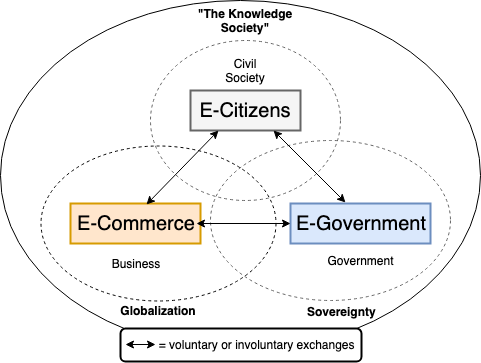
\includegraphics[width=0.7\textwidth]{figuras/relacao_triangular_e-gov.png}
\caption{Modelo de Relacionamento Triangular: Governo Eletrônico, Negócios e Cidadãos. Adaptado de \cite{fang2002government}.}
\label{img:triangulo}
\end{figure}

Neste sentido, o conceito de Governo Digital envolve diversos âmbitos, evidenciando a grandeza e importância de um processo de transformação digital no governo.


\section{Transformação Digital no Brasil}

No Brasil, em 2016, somente 54\% dos domicílios brasileiros possuíam acesso à internet, o que representa 6,7 milhões de residências e um total de 107,9 milhões de usuários de Internet~\cite{CGI}. Neste mesmo ano, ocorreu o lançamento da \textit{Estratégia de Governança Digital da Administração Pública Federal} (EGD), com o objetivo de definir estratégias, metas e indicadores da Política de Governança Digital. A partir da EGD, a prestação de serviços
públicos poderia ser simplificada e agilizada proporcionando uma melhoria no ambiente de negócios e eficiência da gestão pública.

Ainda em 2016, o Decreto número 8.638 foi publicado pela Casa Civil da Presidência da República \cite{BRASIL2016c}, instituindo a Política de Governança Digital, no âmbito dos órgãos e das entidades da administração pública federal direta, autárquica e fundacional. 

% No Decreto número 8.638 \cite{BRASIL2016c}, existem dois artigos a serem destacados por seus princípios e objetivos, estes estão 
% listados na tabela a seguir:

Para estimular a transformação dos serviços públicos em serviços digitais, de modo que estes ocorram por meio eletrônico, o governo
brasileiro publicou decretos relevantes entre 2014 e 2016, como citado ao longo desta seção. Os decretos definiram a Política de Governança
Digital e a Plataforma de Cidadania Digital, no âmbito da Administração Pública Federal (APF), ambos de responsabilidade do então 
Ministério do Planejamento, Desenvolvimento e Gestão (MP) \cite{BRASIL, BRASIL2016}. 

A Plataforma de Cidadania Digital configura um conjunto de metodologias e soluções que buscam ampliar e simplificar o acesso dos cidadãos aos serviços digitais e, também, para apoiar os órgãos públicos na aceleração da transformação digital de serviços.  

Simultaneamente às ações da Plataforma de Cidadania Digital, o Departamento lançou um canal para oferecer informações no
formato de um portal de serviços do Governo Federal\footnote{https://www.servicos.gov.br/}. A iniciativa surgiu para permitir o arquivamento de solicitações eletrônicas e monitorar os serviços públicos pelos usuários. Juntamente com o portal, foi lançado um programa de automação de serviços públicos, para a tentativa de orientar e apoiar órgãos públicos a identificar, priorizar, digitalizar e implementar serviços 
com mais qualidade e transparência para os cidadãos.

Um dos objetivos do governo brasileiro com a transformação digital é ampliar os serviços públicos nos canais digitais. 
Atualmente, o governo oferece aproximadamente 1.700 serviços, mas apenas 41\% são totalmente digitais. Vale ressaltar que o processo de transformação brasileiro envolve os três principais focos apresentados na Figura \ref{img:triangulo}: \textit{E-Government}, \textit{E-Commerce} e \textit{E-Citizens}.

Tendo em vista os decretos publicados, o Departamento \textbf{INOVA} do antigo MP, se responsabilizou pela construção de um programa de Governo Digital, denominado \textit{Kit de Transformação}. O objetivo é, de modo geral, transformar os serviços públicos a partir da utilização de um kit, ao invés da adoção de uma metodologia, por exemplo, objetivando facilitar a adoção e orientação aos diversos órgãos da APF.

O \textit{Kit de Transformação} é composto por seis estágios de aplicações independentes, como demonstrado na Figura \ref{fig:EtapasTransform}.

        \begin{figure}[h]
          \centering
          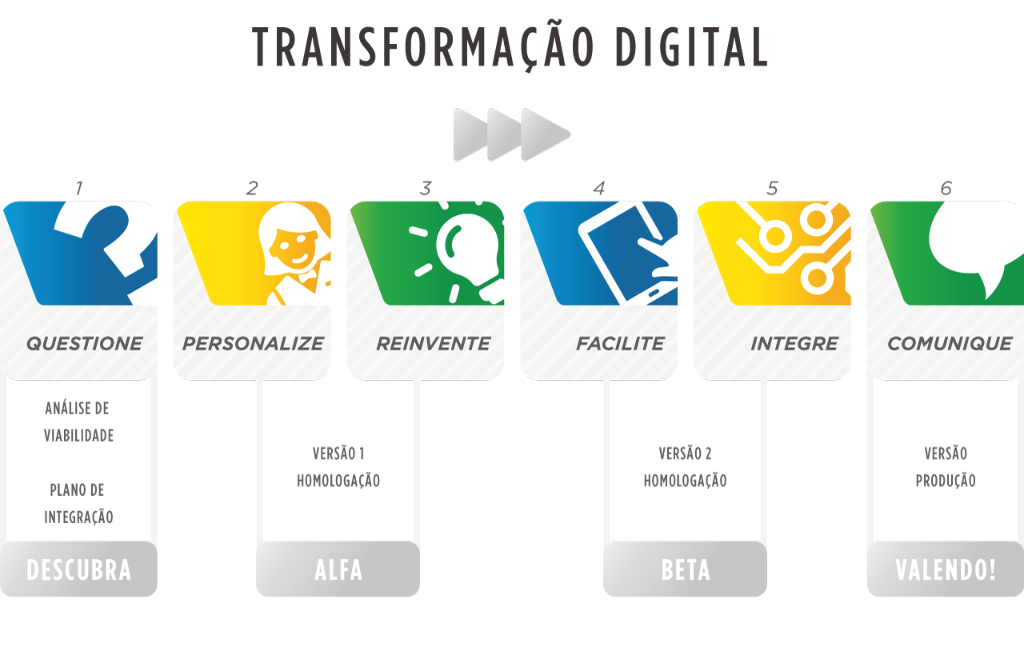
\includegraphics[width=15cm]{figuras/secao-referencial/EtapasTransform.png}
          \caption{Fases do Kit de Transformação (Fonte: \cite{BRASIL2017})} 
          \label{fig:EtapasTransform}
        \end{figure}
        
        
A seguir é apresentado cada um dos estágios destacados na Figura \ref{fig:EtapasTransform}:

\begin{itemize}
\item \textbf{Questione}

Esta fase foi delineada para que o órgão fosse capaz de identificar e priorizar seus principais serviços, além de realizar um diagnóstico que anteceda a transformação, de modo que uma avaliação posterior resulte nos anseios dos usuários. A metodologia desta fase busca, especificamente, a identificação de serviços, avaliação da maturidade da gestão em serviços, levantamento de custos dos usuários do serviço, priorização da transformação de serviços e, por fim, o diagnóstico e avaliação dos serviços.

\item \textbf{Personalize}
Nesta fase é utilizada a visão do usuário como um propósito para que se atinja serviços personalizados, sendo assim, o ministério busca identificar as necessidades do usuário a fundo para que se mapeie as impressões mais relevantes sobre os problemas levantados. A partir do levantamento das necessidades mais relevantes dos usuários, pode-se conseguir dados sobre o acesso, uso, satisfação e expectativas sobre o serviço prestado, além da análise de qualidade do serviço em questão.


\item \textbf{Reinvente}


É importante que a transformação seja analisada, sintetizada, prototipada e testada, por isso, esta fase realiza a definição do Serviço Mínimo Viável (SMV). Partindo desta definição torna-se possível escolher alternativas de solução e possibilidades de se encontrar um melhor trajeto para a iniciação da transformação de serviços. É fundamental nesta fase que se crie novas soluções para aprimorar e estimular o processo de transformação deste contexto.


\item \textbf{Facilite}


A ideia da fase Facilite é oferecer um guia de simplificação de serviços ao participante. É a partir desta fase que se configuram ferramenta de agendamentos, ferramenta de automação de serviços públicos, solução de peticionamento eletrônico do SEI (Sistema Eletrônico de Informações) e solução de atendimento virtual.



\item \textbf{Integre}


Ao solicitar um serviço, o cidadão precisa disponibilizar tempo e custo logístico para obter a apresentar determinados documentos que são requeridos. Sendo assim, o objetivo desta fase é integrar suas bases de dados às plataformas criadas de modo que, o acesso dos cidadãos aos serviços sejam simplificados, com dados unificados. Com a integração das informações dos usuários pode-se eliminar a necessidade de que se apresente dados já cadastrados pelo cidadão, ou seja, as bases do governo que já capturaram determinadas informações, passam a reutilizá-las em diversas situações, minimizando o esforço por parte do cidadão.


\item \textbf{Comunique}


Para que se planeje e comunique aos cidadãos as mudanças realizadas, é necessário que o órgão defina e avalie ações de comunicação. Para tanto, a fase Comunique necessita da transformação do serviço pronta para ser implantada, com seus respectivos canais de atendimento para a transformação do serviços. 

\end{itemize}

Por meio das ferramentas da fase \textit{Questione}, o órgão parceiro poderá avaliar em que medida as ferramentas das demais fases serão úteis para melhorar seus serviços. Com isso, o órgão parceiro terá parâmetros para decidir se utilizará o conjunto completo do Programa ou se adotará uma ``\textit{estratégia de prateleira}'', selecionando aleatoriamente as ferramentas de que necessita.

Para a fase Facilite, o Ministério contratou, por meio de licitações, uma empresa que fornece uma ferramenta de digitalização de serviços baseada no conceito de \textit{meta-design}~\cite{fogli2012meta}. Após a digitalização, os serviços devem ser validados e entregues a população. 

O ITRAC, da UnB, em seu projeto de parceria com o então Ministério do Planejamento, contribuiu para o programa de automatização no quesito da garantia da qualidade dos serviços transformados.



%---------------- Testes Exploratórios-----------------%
\section{Processo de Testes definidos pelo ITRAC}

A busca pela simplificação  e transformação de serviços utilizando das soluções tecnológicas que a empresa terceiriza proporciona está relacionada à problemática de se testar sem requisitos. A transformação digital que se ocorre não garante requisitos estáveis ou, até mesmo, a existência de requisitos e isto pode resultar em um problema definido como Problema do Oráculo~\cite{barr2015oracle}. 

O cenário de requisitos instáveis dificulta a identificação do comportamento atual do serviço digitalizado ao ser comparado com o comportamento esperado, ou ao ser analisado como um comportamento errado.  Além disso, devido a forma de contratação definida, o código-fonte dos serviços transformados não são disponibilizados, o que dificulta mais ainda o processo de testes e a extração de informações por parte da equipe de testes.

Levando todo o contexto da transformação dos serviços em consideração, foi desenvolvido um processo de validação sistematizado, com o intuito de garantira qualidade da digitalização dos serviços. As etapas de criação e execução de casos de teste de cada serviço podem ser realizadas usando diversos padrões de teste, desde estratégias de teste manual até testes automatizados. 

O processo de validação dos serviços digitizados  definido pelo ITRAC está de acordo com o apresentado na Figura \ref{img:process_test}.
 
 \begin{figure}[H]
 \centering
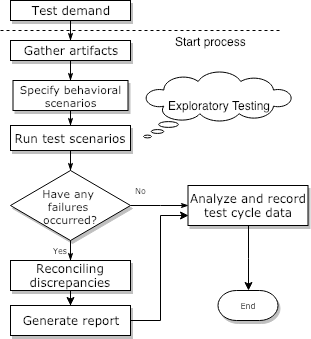
\includegraphics[width=0.7\textwidth]{figuras/Processo_artigo_menor.png}
\caption{Processo de Validação de Serviços definido pelo ITRAC adaptado de~\cite{elcock2006testing}.}
\label{img:process_test}
\end{figure}

Visto que o código-fonte não é acessível pelo ITRAC e o conjunto de requisitos não é bem definido, o processo proposto pelo ITRAC se baseia na estratégia proposta por \cite{elcock2006testing} e no conceito de Teste Exploratório (ET), sugerido por \cite{whittaker2009exploratory}, usando a metáfora do turista como uma estratégia para guiar, através das chamadas ``tours'', a descoberta de requisitos e regras de negócios, além de sistematizar a criação e execução dos casos de teste. O conceito de Testes Exploratórios utilizado como base para definição do processo de teste será apresentado, de maneira detalhada, na Seção \ref{sec:testes_exploratorios}.


A partir da padronização do processo de teste definida pelo ITRAC, foi possível iniciar o desenvolvimento de uma ferramenta de apoio ao processo de teste dos serviços digitizados. A ferramenta, chamada \textit{Digital Transformation Environment Support Tool}, ou DTEST é apresentada a seguir.

\subsection[DTEST]{Ferramenta DTEST -- Digital Transformation Environment Support Tool}
\label{sec:dtest}

A partir da análise das características envolvidas no processo de Transformação Digital brasileiro, foi definida uma ferramenta de apoio ao processo de transformação, representada pela Figura \ref{img:architecture}, a qual tem como objetivo maximizar a eficiência do processo de transformação digital no governo brasileiro.

\begin{figure}[!htb]
\centering
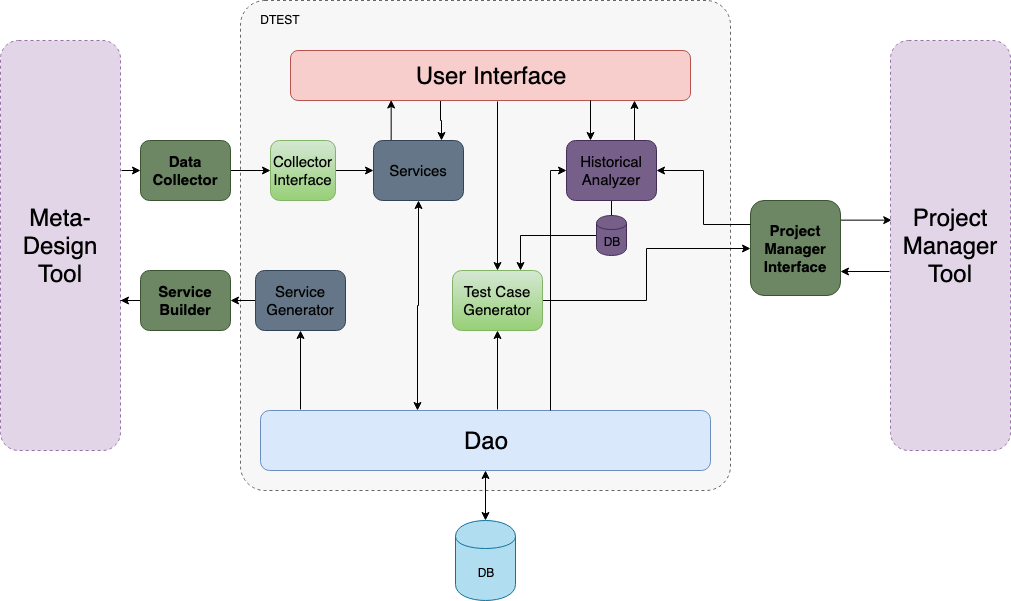
\includegraphics[width=1\textwidth]{figuras/arquitetura_sem_tester.png}
\caption{Arquitetura DTEST (Fonte: Elaborado pela Autora.)}
\label{img:architecture}
\end{figure}

O principal objetivo da ferramenta é facilitar a realização das atividades relacionadas ao processo de Transformação Digital no governo brasileiro. Dessa forma, a \itractool se baseia na utilização de ferramentas geradoras de produtos de software com base em estratégias de meta-design e EUD. Considera-se, também, que ferramentas de gerenciamento de projetos são utilizadas como forma de gerenciamento e acompanhamento das atividades do processo de transformação. Dessa forma, de acordo com o apresentado na Figura \ref{img:architecture}, a \itractool se encontra entre a ferramenta de meta-design e a ferramenta de gerenciamento de projeto utilizada pela equipe de Transformação Digital. 

O componente central da arquitetura apresentada na Figura \ref{img:architecture} agrupa os módulos da \itractool. Os módulos destacados na cor verde escuro, ``Data Collector" e ``Project Manager Interface", são módulos a parte e que devem ser definidos de acordo com o contexto em que a \itractool será utilizada. Esta estrutura de componentes objetiva a aplicabilidade da ferramenta proposta em diversos contextos, garantindo, ainda, a generalidade e replicabilidade do trabalho apresentado.

A seguir são apresentados os principais módulos envolvidos no ambiente da ferramenta \itractool.

\begin{itemize}
    \item O módulo \textit{Data Collector} é responsável pela extração de informações na ferramenta de meta-design. Esta extração pode ser realizada como a equipe desejar. No nosso contexto, a extração precisou ser feita via \textit{web crawler}, mas poderia ser feita via API ou acesso ao banco de dados, por exemplo. A partir da obtenção dos dados, estes são mapeados em entidades do tipo \textit{Service} e registrados no banco de dados para consulta dos próximos módulos. 
    
    \item O módulo \textit{Collector Interface} é responsável por definir as regras de interface para integração do módulo \textit{Data Collector}.
    
    \item O módulo \textit{Services} é responsável pelo gerenciamento do serviços extraídos. Constrói e distribui as relações entre cada entidade dos serviços, estas relações podem ser denominadas e enxergadas no código como \textit{Stages} e \textit{Fields}. Este também é responsável por registrar todas as informações de serviços no banco de dados para consulta de outros módulos. 
    
    % \del{Acho que nesse ponto, ainda não foi dito o que são Stages e Fields. Acredito que, se for o caso, poderia se descrever, quando se fala da ferramenta de Meta-Design, no que consiste um serviço e como o meta-modelo faz esse mapeamento para esclarecer isso.}
    
    \item O módulo \textit{Test Case Generator} é o módulo responsável pela geração automática de casos de teste para validar determinado serviço digitizado.
    
    \item O módulo \textit{Tester Manager} é responsável pelo gerenciamento de atividades de teste. Entre os objetivos deste módulo está a Atribuição de \textit{tours} nesse caso específico para testadores com base em características de ambos testadores e tours.
    
    \item O módulo \textit{Historical Analyzer} é responsável pela análise dos dados históricos para melhoria contínua do processo de transformação. 
    
    \item O módulo \textit{Project Manager Interface} é responsável pela formatação dos dados resultantes para registro na ferramenta de gerenciamento de projeto utilizada pela equipe. Este também é responsável pela extração de informações de gerenciador de projeto para gerar informação para o módulo \textit{Historical Analyzer}.
\end{itemize}

De maneira mais detalhada, as principais funcionalidades presentes na ferramenta são apresentadas a seguir.

\subsubsection{Suporte à Validação}
\label{sec:teste}

A partir da experiência obtida com a garantia da qualidade dos serviços advindos do contexto brasileiro de Transformação Digital, foi possível definir estratégias automatizadas para maximizar a eficiência da atividade de validação. O processo de validação dos serviços se baseia na utilização do conceito de Testes Exploratórios de tal forma que possibilitou a padronização e sistematização dos casos de teste por meio dos tours. A partir desta padronização foi possível criar uma estrutura para geração automatizada de casos de teste com base nas características do SUT.

Como o contexto brasileiro de TD se baseia em estratégias de meta-design e EUD para desenvolvimento do serviços, a extração das características de cada serviço é uma atividade passível de automação. No nosso contexto, foi desenvolvido um script em Python para extração de informação de cada serviço a partir da execução de um \textbf{web crawler} na ferramenta de meta-design utilizada. A partir da obtenção de todas as informações necessárias, é possível fazer a geração automatizada de casos de teste.

A estratégia de extração de informações dos serviços digitizados segue o padrão utilizado pela ferramenta de meta-design adotada pelo governo brasileiro. Deste modo, observa-se que um \textbf{Service} possui uma ou mais \textbf{Stages} e muitos \textbf{Fields}. Entretanto, vale destacar que cada \textbf{Field} está associado a todas as \textbf{Stages} do serviço, entretanto com configurações diferentes (somente leitura, obrigatório, opcional e etc). A partir desta estrutura de relacionamento, o Algorithm \ref{test_case_generation} apresenta a lógica utilizada para geração dos casos de teste com base nas características do SUT.

    \begin{algorithm}[!htb]

	\KwIn{Service service}
	\KwResult{List tests}

	\SetKwProg{Fn}{Function}{}{}
	\Fn{generate\_test\_cases(service)}{
	   tests = []\;
	   
	   \For{service.stages as stage}{
	        tests.append(test\_cancel\_stage(stage))\;
	        
	        \For{stage.stage\_fields as stage\_field}{
	            type = verify\_type(stage\_field)\;
	            tests.append(create\_test(type, stage\_field))\;
	        
	        }
	   }
        % \If{not f\_base}{
        %     feature.save()\;
        % }
		\Return{tests}\;
	}
\caption{Test Case Generation.}
\label{test_case_generation}
\end{algorithm}

A linha 3 do Algoritmo~\ref{test_case_generation} extrai todas as \textbf{Stages} de um serviço e itera sobre elas. Para cada \textbf{Stage}, um caso de teste baseado na Tour Período Chuvoso (Metáfora do Turista \cite{whittaker2009exploratory}) é gerado, validando o funcionamento correto da opção de cancelar a \textbf{Stage} atual.

Outros casos de teste genéricos para qualquer \textbf{Stage} devem ser incluídos após a linha 3 e antes da linha 5. Após a linha 5 do Algoritmo~\ref{test_case_generation}, cada relação Stage-Field é analisada para geração de casos de teste específicos com base na configuração de cada \textbf{Field} em cada \textbf{Stage}. Com esta estrutura, basta identificar casos de teste adequados a determinadas características do serviço e incluí-lo como uma nova verificação dentro do método \textit{create\_test()}. A Tabela~\ref{tab:test_types} apresenta os tipos de teste já cobertos pela \textbf{ITRACtool}.


\begin{table}[htb!]
\centering
\caption{Current types of auto-generated test cases.}
\label{tab:test_types}
\begin{tabular}{|c|c|c|}
\hline
\textbf{Field Type}                                                                   & \textbf{Test Case}                                                       & \textbf{Description}                                                                                                                                            \\ \hline
\textit{\begin{tabular}[c]{@{}c@{}}Required \\ Field\end{tabular}}                    & \begin{tabular}[c]{@{}c@{}}Test required \\ fields\end{tabular}          & \begin{tabular}[c]{@{}c@{}}Validate the exception \\ obtained with the \\ submission of the form \\ without the inclusion of \\ the required field\end{tabular} \\ \hline
\multirow{2}{*}{\textit{\begin{tabular}[c]{@{}c@{}}Normal \\ (Visible)\end{tabular}}} & \begin{tabular}[c]{@{}c@{}}Test help \\ text\end{tabular}                & \begin{tabular}[c]{@{}c@{}}Validate the help \\ text message in\\ each visible Field.\end{tabular}                                                              \\ \cline{2-3} 
                                                                                      & \begin{tabular}[c]{@{}c@{}}Test field \\ label\end{tabular}              & \begin{tabular}[c]{@{}c@{}}Verify field label \\ consistency\end{tabular}                                                                                       \\ \hline
\textit{Email}                                                                        & \begin{tabular}[c]{@{}c@{}}Test email \\ field\end{tabular}              & Validate invalid email                                                                                                                                          \\ \hline
\multirow{2}{*}{\textit{Data}}                                                        & \begin{tabular}[c]{@{}c@{}}Test Date \\ field\end{tabular}               & Validate invalid Date                                                                                                                                           \\ \cline{2-3} 
                                                                                      & \begin{tabular}[c]{@{}c@{}}Test Date \\ modal\end{tabular}               & \begin{tabular}[c]{@{}c@{}}Validate the date \\ modal format\end{tabular}                                                                                       \\ \hline
\multirow{4}{*}{\textit{Template}}                                                    & \begin{tabular}[c]{@{}c@{}}Test \\ template\end{tabular}                 & \begin{tabular}[c]{@{}c@{}}Submit an invalid format \\ or size\end{tabular}                                                                                     \\ \cline{2-3} 
                                                                                      & \begin{tabular}[c]{@{}c@{}}Test \\ template\\ specification\end{tabular} & \begin{tabular}[c]{@{}c@{}}Validate the\\ required file specification\end{tabular}                                                                              \\ \cline{2-3} 
                                                                                      & \begin{tabular}[c]{@{}c@{}}Test template \\ size\end{tabular}            & \begin{tabular}[c]{@{}c@{}}Validate the max \\ size accepted\end{tabular}                                                                                       \\ \cline{2-3} 
                                                                                      & \begin{tabular}[c]{@{}c@{}}Test template\\ modal\end{tabular}            & \begin{tabular}[c]{@{}c@{}}Validate the template \\ modal format\end{tabular}                                                                                   \\ \hline
\textit{Phone}                                                                        & \begin{tabular}[c]{@{}c@{}}Test mask\\ phone\end{tabular}                & \begin{tabular}[c]{@{}c@{}}Verify valid and invalid \\ masks for phones\end{tabular}                                                                          \\ \hline
\end{tabular}
\end{table}

Desse modo, o serviço analisado passa por uma inspeção que busca características específicas do serviço para geração de casos de teste. Como resultado da atividade de geração de casos de teste, encontra-se uma lista de casos de teste formatados de tal forma que seja possível a inclusão destes em uma ferramenta de gerenciamento de projetos, para registro e acompanhamento do caso de teste.

\subsubsection{Generation Support}
\label{sec:geracao}

% Dado que a transformação do serviços é feita a partir da utilização de ferramentas de meta-design, é possível identificar pontos de automação que possibilite maximizar a eficiência desta atividade. 
De acordo com a experiência obtida ao longo do primeiro ano de transformação digital, algumas atividades mecânicas puderam ser destacadas, como a construção do serviço, criando as \textbf{Stages} e \textbf{Fields} associados, assim como a configuração de cada \textbf{Field} em suas respectivas \textbf{Stages}. Esta atividade mecânica e repetitiva foi automatizada a partir da implementação dos módulos \textit{``Service Generator"} e \textit{``Service Builder"}, apresentados na Figura \ref{img:architecture}.

Este objetivo é alcançado a partir da definição das características do serviço desejado utilizando a \itractool, exportando essas características para a ferramenta de meta-design. A estratégia adotada para exportar o serviço foi a utilização de um \textbf{web crawler} escrito em Python, responsável por navegar pela ferramenta de meta-design e criar as \textbf{Stages} necessárias, seus respectivos \textbf{Fields} e, consequentemente, suas configurações de visualização e comportamento.

Vale ressaltar que a estratégia de geração de serviços na ferramenta de meta-design deve ser definida de acordo com as características envolvidas. Em alguns casos, algumas adaptações devem ser realizadas, de acordo com o funcionamento da ferramenta de meta-design utilizada pela equipe de transformação.

% Os conceitos utilizados para a definição da estratégia dos testes serão descritos nas seções x, y e z.

De acordo com o apresentado nesta seção, a ferramenta \itractool trabalha com diversas informações úteis para o contexto analisado nesta pesquisa. Dessa forma, a proposta de abordagem apresentada neste trabalho deverá se relacionar com a ferramenta \itractool.

\section{Testes Exploratórios}
\label{sec:testes_exploratorios}

 No contexto do ciclo de vida do desenvolvimento de software, a atividade de teste é de suma importância, visto a sua capacidade de avaliar e melhorar a qualidade do software \cite{bertolino2007software}. Existem diversas técnicas para cumprir o teste sistemático de software, seja teste caixa preta, caixa branca e caixa cinza. Dessa forma, testadores utilizam diferentes técnicas para encontrar e solucionar defeitos com o menor esforço possível \cite{maldonado2004introduccao}. 

A realização de teste por parte de testadores humanos é relevante no desenvolvimento de software do mundo real por facilitar a identificação de novos BUGs, especialmente no contexto de sistemas interativos. Testadores humanos têm vantagens sobre máquinas, visto a capacidade de conhecimento, aprendizado e adaptação a novas situações, que facilita o processo de reconhecimento eficiente de dos problemas~\cite{itkonen2015test}. 

O ato de explorar pode ser consolidado quando não se sabe ao certo qual caminho traçar para se chegar a determinado ponto, este ato é análogo ao teste de software, porque busca descobrir informações sobre a qualidade do sistema a ser testado~\cite{itkonen2015test}.

O Teste Exploratório (TE) é uma abordagem de teste manual que emerge com um potencial de adaptação para os testes a partir de um processo de aprendizagem, utilizando de uma visão mais humana e relacionada à experiência dos envolvidos. Esta abordagem de teste foi mostrada na indústria de software com seus primeiros materiais produzidos aparecendo em blogs da internet~\cite{kaner2000testing} e, em 2009, aparecendo em livros e artigos. 

O termo também aparece em \textbf{SWEBOK}~\cite{bourque2014guide}, onde é definido simultaneamente como aprendizagem, o projeto de teste 
e a execução do teste, ou seja, os testes são definidos antecipadamente em um plano de teste estabelecido, mas 
são dinamicamente projetados, executados e modificados.

Por meio do teste exploratório, é possível que o testador não dependa de um conjunto de casos de teste pré-projetados, visto que, dentro dessa abordagem de teste existem etapas de \textit{design} e execução de testes, nas quais os testadores estão constantemente aprendendo e 
adaptando suas atividades. De maneira prática, o testador aprende iterativamente sobre o produto e suas falhas, projeta e executa os testes de forma dinâmica~\cite{whittaker2009exploratory}, mas sistemática. Os tours permitem aos testadores se recordarem dos objetivos do teste e, desse modo, mesmo que os testes sejam feitos de forma manual e exploratória, a forma de exploração fica sistematizada quando testador procura atingir o objetivo do tour.

A Tabela~\ref{tab:comparativo} apresenta uma adaptação da comparação realizada por \cite{itkonen2015test}, na qual se observa a repetibilidade mecânica, orientada por documentos na execução do teste. A abordagem de testes exploratórios destaca o conhecimento, a aprendizagem e a descoberta de novas informações que proporcionam um conhecimento mais aprofundado do software. 

O teste exploratório apresenta objetivos semelhantes aos testes automatizados, entretanto, o TE não utiliza descrições formais ou metodologias detalhadas, além da não necessidade de acesso ao código-fonte, o que faz com que sua abordagem seja mais adequada ao contexto da transformação digital de serviços, parte deste trabalho. 

% Please add the following required packages to your document preamble:
% \usepackage{graphicx}
% \usepackage[table,xcdraw]{xcolor}
% If you use beamer only pass "xcolor=table" option, i.e. \documentclass[xcolor=table]{beamer}
\begin{table}[!htb]
\caption{Comparativo entre teste automatizado, teste manual (\textit{ad-hoc}) e teste exploratório. Adaptado de \cite{itkonen2015test}.}
\label{tab:comparativo}
\resizebox{\textwidth}{!}{%
\begin{tabular}{|l|l|l|l|}
\hline
\rowcolor[HTML]{333333} 
{\color[HTML]{FFFFFF} } & {\color[HTML]{FFFFFF} \textbf{Automatizado}} & {\color[HTML]{FFFFFF} \textbf{Manual (ad-hoc)}} & {\color[HTML]{FFFFFF} \textbf{Teste Exploratório}} \\ \hline
\rowcolor[HTML]{FFFFFF} 
\textbf{\begin{tabular}[c]{@{}l@{}}Filosofia \\ de Teste\end{tabular}} & Automatizado e repetitivo para oferecer feedback & \begin{tabular}[c]{@{}l@{}}Mecânico, repetitivo \\ e descrito em instruções explícitas.\end{tabular} & \begin{tabular}[c]{@{}l@{}}Conhecimento intensivo,\\ atividade criativa que requer habilidades.\end{tabular} \\
\rowcolor[HTML]{EFEFEF} 
\textbf{\begin{tabular}[c]{@{}l@{}}Design \\ de Teste\end{tabular}} & \begin{tabular}[c]{@{}l@{}}Design desafiador e caro, \\ mas de execução rápida e barata.\end{tabular} & Design separado e sequencial. & \begin{tabular}[c]{@{}l@{}}Design e execução paralelos; \\ Requer aprendizagem exploratória \\ do teste.\end{tabular} \\
\rowcolor[HTML]{FFFFFF} 
\textbf{Documentação} & \begin{tabular}[c]{@{}l@{}}Certos tipos de testes podem ser \\ roteirizados e automatizados.\end{tabular} & \begin{tabular}[c]{@{}l@{}}O teste pode ser distribuído para\\ diversos tipos de pessoas \\ com base nos testes documentados.\end{tabular} & \begin{tabular}[c]{@{}l@{}}Requer conhecimento e habilidades\\ difíceis de transferir com\\ a documentação.\end{tabular} \\
\rowcolor[HTML]{EFEFEF} 
\textbf{\begin{tabular}[c]{@{}l@{}}Conhecimentos \\ Necessários\end{tabular}} & \begin{tabular}[c]{@{}l@{}}Certos tipos de bugs podem ser \\ efetivamente detectados\\ automaticamente.\end{tabular} & \begin{tabular}[c]{@{}l@{}}Previsão de erros;\\ Resultados esperados documentados \\ para simples comparação de \\ tempo de execução.\end{tabular} & \begin{tabular}[c]{@{}l@{}}Os bugs são imprevisíveis e requerem\\ conhecimento do sistema e do domínio\\ da aplicação para detecção.\end{tabular} \\
\rowcolor[HTML]{FFFFFF} 
\textbf{Repetibilidade} & \begin{tabular}[c]{@{}l@{}}Repetibilidade e execução de testes em ciclos \\ muito curtos, mecessita de feedback rápido \\ sobre a regressão durante o desenvolvimento.\end{tabular} & \begin{tabular}[c]{@{}l@{}}Repetibilidade essencial; \\ Descrições exatas de casos de teste reduzem \\ a variação individual nos testes.\end{tabular} & \begin{tabular}[c]{@{}l@{}}Repetir os mesmos testes \\ não revela novos bugs nem\\ novas informações sobre a qualidade,\\ oferecendo pouco valor agregado.\end{tabular} \\
\rowcolor[HTML]{EFEFEF} 
\multicolumn{1}{|c|}{\cellcolor[HTML]{EFEFEF}\textbf{Automatização}} & \begin{tabular}[c]{@{}l@{}}Os testes devem ser \\ automatizados o máximo possível.\end{tabular} & \begin{tabular}[c]{@{}l@{}}Testadores humanos podem ser usados\\ para objetivos semelhantes aos da automação.\end{tabular} & \begin{tabular}[c]{@{}l@{}}A automação deve ser usada \\ para aprimorar os testes \\ e liberar recursos humanos para outros \\ tipos de atividades de teste.\end{tabular} \\ \hline
\end{tabular}%
}
\end{table}

\subsection{Metáfora do Turista}

Para sistematizar o processo de TE, \cite{whittaker2009exploratory} propôs a Metáfora do Turista, a qual consiste na analogia entre um turista em uma cidade e o teste de software. Segundo \cite{whittaker2009exploratory}, o turismo é uma mescla entre estrutura e liberdade, assim como o teste exploratório. Dessa forma, ele definiu a metáfora do turista com o objetivo de auxiliar na construção dos testes.

Na analogia apresentada, as funcionalidades dos softwares são separadas em distritos, que significam a delimitação de um espaço que se decide explorar, o que, na prática, representa as diferentes áreas do software. Além disso,  cada distrito possui um conjunto de ``tours'', que representam as diferentes maneiras de percorrer as diferentes características e funcionalidades do software. A seguir, são destacados alguns dos distritos mais utilizados pela equipe e suas respectivas ``tours'':

\subsubsection{Distrito Hoteleiro}

 É geralmente onde o turista descansa depois de um dia cheio de passeios e fica longe da agitação da viagem. Em um software, esse distrito representa os recursos secundários do aplicativo, normalmente ignorados ou deixados de lado. Em relação a este distrito, as ``tours'' utilizadas neste trabalho de pesquisa foram:

\begin{itemize}
    \item \textbf{Tour em Período Chuvoso}: Um turista pode se encontrar em um dia chuvoso e sentir vontade de tornar o passeio mais curto ou até mesmo cancelá-lo. No software, a recomendação é que o testador, ao fazer as ``tours'', use as opções que interrompem o processo do sistema. Os recursos que exigem processamento de intervalo de tempo e fornecem uma opção de cancelamento durante o preenchimento de algumas informações devem ser iniciados e cancelados, com o objetivo de verificar se as opções de cancelamento funcionam adequadamente em qualquer contexto.
    
    \item \textbf{Tour com Desinteressados}: Ao passear em uma cidade turística, alguns turistas podem parecer preguiçosos e desinteressados, não curtindo o passeio e o guia turístico pode ter que se esforçar mais para entretê-los. No contexto do software, os testadores desinteressados podem ser muito eficazes. A ``tour'' consiste em fazer o sistema funcionar fornecendo o mínimo de dados possível, forçando-o a se alinhar com valores padrão e entradas vazias.
\end{itemize}

\subsubsection{Distrito Decadente} 

Local onde costumam ocorrer alarmes constantemente. No software, essas ``tours'' têm como objetivo fornecer ações que podem causar falhas no software. As ``tours'' utilizadas nesta pesquisa foram:

\begin {itemize}
    \item \textbf {Tour Sabotador}: Todas as oportunidades para sabotar o aplicativo devem ser usadas. Nesta ``tour'', o testador deve forçar o software a iniciar alguma operação, identificar os recursos necessários para terminá-lo e remover esses recursos. Deve-se, por exemplo, solicitar que o aplicativo leia algo no disco, mas sabotar a tentativa de leitura para causar confusão, levando o sistema a falhar.
    \item \textbf {Tour Antissocial}: Em um passeio pela cidade, o turista anti-social é aquele que mostra claramente a insatisfação com o passeio e faz questão de encontrar algo para se opor a tudo o que é visto ou falado durante o passeio. Para testadores, é indispensável ter esse aspecto anti-social, com o objetivo de procurar por todos os tipos de possíveis falhas no software. A ``tour'' anti-social consiste em inserir entradas que nunca devem ser inseridas e/ou entradas que possam causar danos ao sistema.
\end {itemize}

\subsubsection{Distrito de Negócios}

É aquele em que bancos, lojas, blocos comerciais e restaurantes podem ser encontrados. Em suma, é o distrito que tem o horário comercial produtivo e as interações sociais típicas do pós-trabalho. Fazendo uma associação com software, o Distrito de Negócios é o núcleo do aplicativo, com os principais recursos que o usuário recorre no sistema. Neste distrito, as seguintes ``tours'' foram selecionadas:

\begin {itemize}
    \item \textbf {Tour Intelectual}: Os guias turísticos estão sujeitos a responder perguntas difíceis, formuladas pelos turistas com uma combinação de curiosidade e conhecimento prévio do local visitado. Para os testadores, \textit{The Intellectual Tour} consiste em uma sobrecarga do software do modo que requer mais processamento ou faz com que sua capacidade de trabalho em situações hostis seja testada.
    \item \textbf {Tour FedEx}: A FedEx é uma das maiores empresas de entrega de encomendas do mundo e faz todo o trabalho de coleta e distribuição desses pacotes para que cheguem ao seu destino final. A \textit{FedEx Tour} é baseada na noção de verificação de movimentação de dados dentro do aplicativo, testando se há algum tipo de corrupção durante esse caminho.

    \item \textbf {Tour Coletor de Lixo}: Os coletores de lixo percorrem a cidade de maneira metódica, e como resultado disso eles estão bem familiarizados com os lugares em que normalmente são alterados. O \textit{Garbage Collector Tour} consiste no testador executar o aplicativo inteiro para um propósito específico e de maneira metódica. Um exemplo seria verificar todas as mensagens de erro ou aviso fornecidas em todos os recursos do sistema.
    \item \textbf {Tour Guiado (F1)}: Guias de viagem orientam os turistas sobre os melhores lugares e atrações da cidade visitada. Trazendo-o ao contexto do software, os guias referem-se aos manuais do usuário. Também chamado de ``F1 Tour'', o Tour Guiado induz o testador a usar manuais do usuário para ajudar a explorar o software de acordo com o que eles indicam.
\end {itemize}

\subsubsection{Distrito Histórico}

É onde estão os edifícios da cidade antiga, os lugares de relevância histórica que são geralmente pontos turísticos muito populares. No software, o distrito histórico representa localizações de códigos legados, recursos mais antigos e falhas corrigidas. Apenas uma ``tour'' foi selecionada neste distrito para esta pesquisa:

\begin{itemize}
    \item \textbf {Tour à Vizinhança Ruim}: As áreas que os turistas são aconselhados a evitar existem em todas as cidades, principalmente devido a perigos e problemas estruturais da cidade. O objetivo desta ``tour'', quando nos referimos ao contexto de software, é averiguar áreas do software que costumam apresentar um alto número de defeitos. Assim, o testador se concentra mais em áreas onde a identificação de defeitos é mais provável.
\end{itemize}

%falar sobre a LECOM, fazer um overview sobre a empresa e a relação dela com o ministério, depois relacionar com a necessidade do processo de validação

% fazer um comparativo entre LECOM e Apex, só a fim de citar uma outra empresa que presta serviços pro governo.

% incluir a figura de representação do serviço digital 

%---------------- Perfil de Testadores--------------%

Como já foi levantado anteriormente, características pessoais dos testadores são atributos importantes quando se refere ao contexto de Testes Exploratórios, como mostram \cite{whittaker2009exploratory, itkonen2015test, itkonen2012role, itkonen2005exploratory}. Dessa forma, a Seção~\ref{sec:perfil_testadores} apresenta uma discussão importante sobre o perfil de testadores e seu impacto no processo de desenvolvimento, verificação e validação de software.

%---------------- Perfil de Testadores -----------------%
\section{Perfil de Testadores}
\label{sec:perfil_testadores}


A atividade de teste é essencial dentro do contexto da Engenharia de Software, podendo assegurar a qualidade do produto de software a partir da identificação de defeitos no software~\cite{myers2004art}. Nas últimas décadas, têm sido estabelecidas técnicas, critérios, métodos
e ferramentas para suportar o processo de desenvolvimento de software, a fim de acompanhar a crescente utilização da tecnologia por parte da população como um todo~\cite{maldonado2004introduccao}.

Existe uma vasta quantidade de ferramentas que auxiliam na examinação do software e, a partir da examinação diretamente do software em execução, o teste fornece um \textit{feedback} de comportamentos reais, que o torna o complemento inevitável de outras técnicas de análise e garantia de qualidade na indústria. Entretanto, esta atividade ainda pode exigir muito trabalho humano, apesar da comunidade científica considerar mais a utilização de testes automatizados~\cite{bertolino2007software}.

Nos últimos 50 anos, a Engenharia de Software se preocupa com a influência da personalidade humana em tarefas individuais de trabalho, como aponta a revisão sistemática de literatura feita por~\cite{cruz2011personality}. Esta preocupação dá origem a pensamentos sobre como traçar estratégias para que se possa usar a análise da personalidade para a prática da Engenharia de Software. 

Os trabalhos publicados e citados sobre testes exploratórios permitem concluir que a personalidade humana pode ter influência sobre este método de teste~\cite{bach2003exploratory, whittaker2009exploratory, itkonen2015test, itkonen2012role, shoaib2009empirical}. As ações de testadores durante a aplicação de testes exploratórios podem variar significativamente de uma pessoa para outra, isto é, a metodologia adotada por testadores tem relação direta com os traços da personalidade de cada testador~\cite{shoaib2009empirical}. 

O trabalho de \cite{shoaib2009empirical} realizou um experimento projetado para identificar os testadores que podem alcançar o melhor resultado durante a aplicação de testes exploratórios. O trabalho se baseou em pré e pós-testes, sendo que, para testar a hipótese da pesquisa, um \textit{Teste de Aptidão de Teste Exploratório} (ETAT) foi realizado em um conjunto de testadores (amostra) para provar a influência da personalidade na aplicação dos testes. Os resultados do experimento mostram existência de uma relação positiva entre o teste exploratório e traços da personalidade humana. Em particular, os testadores que apresentaram uma personalidade extrovertida foram os mais propensos a serem bons testadores exploratórios.

As organizações estão adotando várias metodologias e forças de trabalho alternativas para realizar as entregas de software de maneira eficiente~\cite{dubey2017personas}. Traçar estratégias para que se estruture a equipe adequada para realização da atividade de teste é uma tarefa que pode reforçar estas forças de trabalho e garantir uma entrega mais ágil sem que se comprometa a qualidade do produto de software.

Embora a atividade de testes seja a solução para assegurar um produto ou serviço de software confiável, a execução dos casos de teste pode configurar um trabalho desinteressante se comparado ao projeto ou à codificação. Principalmente quando nos referimos a testes manuais exploratórios. E, sendo uma atividade baseada em humanos, os resultados de um produto de software são dependentes de fatores humanos e carregam desafios para as equipes de desenvolvimento de software, um exemplo de desafio é a busca por uma forma mais eficaz de aumentar a motivação e a satisfação dos testadores~\cite{deak2016challenges}.

Por outro lado, \cite{berner2005observations} afirma em seu trabalho que os testes automatizados nunca podem substituir completamente os testes manuais. \cite{martin2007good} também apresentou relatórios, em seu trabalho, que afirmam que os problemas relacionados ao teste de software na indústria estão relacionados com o ambiente sociotécnico e estrutura organizacional da empresa. Ou seja, os problemas enfrentados na atividade de teste não estão, necessariamente, associados apenas à causas técnicas.

A relação entre teste de software e aspecto humano foi estudada por~\cite{shah2010studying} no contexto de uma empresa baseada em serviços, na qual foi observada a dimensão humana em aspectos como atitude e motivação e aspectos sociais no teste de software. Neste estudo, foram coletadas informações sobre as atitudes dos participantes em relação ao teste de software. Estas foram separadas em categorias baseadas no nível de expertise do indivíduo utilizando os níveis \textit{sênior} e \textit{júnior}. 

% \del{``onde'' deve ser utilizado apenas no sentido de lugar. Os outros usos não são corretos, ok?}
 
Dentro dos dois grandes grupos separados por \cite{shah2010studying}, para os profissionais \textit{sêniors}, a atividade de teste é considerada importante, porém, enfadonha, o que os fazem compartilhar com profissionais imaturos a necessidade e os benefícios de se testar. Além disso, alguns dos participantes do estudo realizado relataram a correlação entre a prática do teste de software como um aprendizado para se aprimorarem em suas atividades de desenvolvimento.

Já os profissionais \textit{juniores}, que possuíam dois anos ou menos de experiência, relataram terem adquirido um vasto aprendizado sobre o sistema no qual estavam trabalhando, visto que, após trabalharem com a atividade de testes, perceberam a importância da coerência do código e o impacto positivo que os testes podem ter na garantia da qualidade. Além disso, os resultados sobre a pesquisa mostrou que as atitudes de profissionais mais antigos podem influenciar significativamente atitudes de pessoas que não possuem uma vasta experiência. 

\cite{ekwoge2017tester} apresentaram em seu trabalho vários tipos de utilizações para o termo ``experiência'' no contexto dos papéis da Engenharia de Software, incluindo: 

% \del{Preste a atenção que, quando a referência for de mais de um autor ou et al, a concordância deve ser no plural}

\begin{itemize}
    \item  \textit{Experiência do Usuário}, que está relacionada ao ponto de vista de uma pessoa diante do uso antecipado de um produto, sistema ou serviço~\cite{hassenzahl2008user};
    \item  \textit{Experiência do Desenvolvedor}, que consiste nas experiências do desenvolvedor sobre todos os tipos de artefatos e atividades relacionadas a ele~\cite{fagerholm2012developer};
    \item  \textit{Experiência do Cliente}, que baseia-se na interação do cliente com o fornecedor do produto ou serviço~\cite{palmer2010customer};
    \item \textit{Experiência de Marca}, que se refere à respostas do cliente e respostas comportamentais evocadas por estímulos relacionados que fazem parte do design e da identidade da marca, embalagem, comunicações e ambiente~\cite{brakus2009brand}.
\end{itemize}

A experiência do testador se relaciona com os artefatos que se busca testar e com às atividades de teste relacionadas a ele. Como os artefatos que serão testados são resultado de um processo de implementação realizado pela equipe de desenvolvimento, pode-se concluir que a atividade de teste é impactada, também pela experiência dos desenvolvedores que geraram estes artefatos.

O estudo de caso realizado por \cite{itkonen2015test} evidencia a experiência do testador com os TEs como uma maneira natural de se fazer testes, justificando a atividade de explorar como uma ação que enfatiza a utilização da experiência e criatividade dos testadores para encontrar defeitos durante a execução dos testes. 

Neste sentido, como já abordado por~\cite{cruz2011personality}, o desempenho da equipe pode variar a depender de seus membros e de suas respectivas características de personalidade e experiência. Esta narrativa contribui fortemente para o contexto do presente trabalho, tendo em vista que o laboratório da universidade (ITRAC) é um ambiente composto por equipes volúveis.



%---------------- Sistema de Recomendação--------------%
\section{Sistemas de Recomendação}
\label{sec:sistemas}

Sistemas de Recomendação (SRs) buscam fornecer assistência, de forma automatizada, a determinadas tarefas~\cite{adomavicius2005toward}. Os SRs oferecem a possibilidade de se coletar informações sobre as preferências
de seus usuários para um conjunto de itens, podendo ser relacionados a comércio eletrônico, entretenimento, aplicativos, sites e etc~\cite{bobadilla2013recommender}.

O interesse em pesquisas relacionadas à Sistemas de Recomendação (SRs) começaram a surgir em meados de 1990 e tiveram sua ascensão na última década como uma história de sucesso relacionada à área de aplicação de Inteligência Artificial (IA)~\cite{felfernig2008constraint}.  Os SRs podem trazer alguns benefícios e continuar despertando interesse atualmente, tanto na comunidade acadêmica, quanto na comunidade industrial devido à comodidade que suas aplicações práticas proporcionam a usuários~\cite{champiri2015systematic}. 

Nos últimos anos, aplicativos desenvolvidos que buscam auxiliar usuários a buscarem por informações de seus interesses têm se preocupado em como refinar determinadas informações para seus públicos~\cite{adomavicius2005toward}. Esta preocupação em refinar buscas para usuários é relevante quando consideramos a quantidade de informações expostas aos usuários de aplicativos e tecnologias, em geral. Adomavicius et. al~\cite{adomavicius2005toward} afirmou, ainda em 2005, que os SRs poderiam auxiliar os usuários a lidarem com excesso de informações e fornecer recomendações personalizadas de conteúdos e serviços para eles.

Em geral, perfis de usuário são utilizados como filtros para fluxos de documentos para que as preferências de informações dos usuários possam ser usadas para definir perfis de usuários. ~\cite{burke2007hybrid}. Com base nesses perfis traçados, é possível que os SRs tratem as informações e forneçam o que houver de mais relevante àquele perfil. Entretanto, a coleta de informações na internet é uma atividade complexa que precisa ser melhorada a partir do tratamento dessas informações~\cite{porcel2010dealing}.

Durante a atividade de recomendação, há uma fase denominada de \textit{feedback de relevância}, esta fase atua como um processo cíclico em que o feedback dos usuários sobre as decisões do sistema e, a partir disso, as informações recuperadas anteriormente pelo sistema para gerar a recomendação pode ser automaticamente atualizada, de acordo com os perfis de usuário\cite{porcel2010dealing}.

OS SRs propõem recomendações a partir da geração de métodos de recomendação, que geralmente são classificados em três categorias principais: abordagens de recomendação baseadas em conteúdo, abordagens colaborativas e abordagens híbridas. A tabela abaixo foi adaptada do trabalho de~\cite{adomavicius2005toward} e apresenta um balanceamento das abordagens de recomendação com suas respectivas técnicas.

% Please add the following required packages to your document preamble:
% \usepackage{multirow}
% \usepackage[table,xcdraw]{xcolor}
% If you use beamer only pass "xcolor=table" option, i.e. \documentclass[xcolor=table]{beamer}
\begin{table}[htb!]
\centering
\begin{tabular}{|l|l|l|}
\hline
 & \multicolumn{2}{l|}{\textbf{Técnica de Recomendação}} \\ \cline{2-3} 
\multirow{-2}{*}{\textbf{\begin{tabular}[c]{@{}l@{}}Abordagem \\ de Recomendação\end{tabular}}} & \textbf{Baseada em heurística} & \textbf{Baseada em modelo} \\ \hline
\rowcolor[HTML]{FFFFFF} 
\textbf{\begin{tabular}[c]{@{}l@{}}Baseada \\ em Conteúdo\end{tabular}} & \begin{tabular}[c]{@{}l@{}}- TF-IDF \\ (recuperação de informação)\\ \\  - Clustering\end{tabular} & \begin{tabular}[c]{@{}l@{}}- Classificador bayesiano\\ \\ - Clustering\\ \\ - Árvores de decisão\\ \\ - Redes Neurais Artificiais\end{tabular} \\ \hline
\rowcolor[HTML]{EFEFEF} 
\textbf{\begin{tabular}[c]{@{}l@{}}Filtragem \\ Colaborativa\end{tabular}} & \begin{tabular}[c]{@{}l@{}}- "Vizinhos mais próximos"\\ \\ \\ - Clustering\\ \\ \\ - Teoria dos Grafos\end{tabular} & \begin{tabular}[c]{@{}l@{}}- Redes bayesianas\\ \\ \\ - Clustering \\ \\ \\ - Redes Neurais Artificiais\\ \\ \\ - Regressão Linear\\ \\ \\ - Modelos Probabilísticos\end{tabular} \\ \hline
\rowcolor[HTML]{FFFFFF} 
\textbf{Híbrida} & \begin{tabular}[c]{@{}l@{}}Combinando conteúdo e\\ componentes colaborativos \\ usando:\\ \\ - Combinação linear de \\ classificações previstas\\ \\ - Esquemas variados de votação\\ \\ - incorporação de um componente \\ como parte da heurística\\ para o outro\end{tabular} & \begin{tabular}[c]{@{}l@{}}Combinando conteúdo e\\ componentes colaborativos\\ por:\\ \\ - incorporação de um componente \\ como parte do modelo para o outro\\ \\ - construção de um modelo unificado\end{tabular} \\ \hline
\end{tabular}
\end{table}

As abordagens expostas na tabela configuram critérios que podem influenciar a aceitação do usuário que terá seus itens recomendados. As subseções a seguir apresentam algumas descrições sobre cada uma dessas abordagens.

\subsection{Filtragem Baseada em Conteúdo (FBC)}

Esta abordagem representa a recomendação realizada baseada em escolhas feitas pelo usuário, de modo que sejam recomendados itens semelhantes aos que o usuário preferiu no passado~\cite{lang1995newsweeder}. Por exemplo, um comércio eletrônico que recomenda filmes aos usuários, baseado em gêneros de filmes que ele comprou anteriormente.

As FBCs podem analisar determinados conteúdos de objetos destinados à recomendação, como por exemplo, textos, imagens e sons que acompanham o conteúdo principal analisado. Seguindo esta análise, o sistema pode detectar semelhanças entra os objetos analisados e recomendar itens semelhantes aos que o usuário comprou, visitou, ouviu e classificou positivamente~\cite{paulson2003combining}. 

Esta abordagem de recomendação têm emergido recentemente devido ao aumento das redes sociais~\cite{bobadilla2013recommender}. O RS apresenta uma tendência a se permitir com que o usuário introduza conteúdos para estabelecer relações sociais, por exemplo, a partir de comentários, críticas, classificações e emissão de opiniões, em geral~\cite{arazy2009improving}. 

Informações adicionais introduzidas pelo usuário podem aumentar a precisão das previsões e recomendações, como apresentado nos trabalhos de~\cite{kim2011collaborative}, \cite{zheng2011recommender} e ~\cite{carrer2012social}. No trabalho de~\cite{kim2011collaborative}, por exemplo, há a incorporação de características colaborativas em um método de recomendação baseado, também, em filtragem de conteúdo que utiliza informações de classificação e informações de marcação, utilizando a noção do trabalho de~\cite{de2008integrating}.

Em resumo, a FBC se baseia no conceito de que itens com atributos semelhantes serão classificados de forma semelhante. Esta abordagem, está se tornando mais importante à medida que o SRs incorporam informações sobre itens de usuários que trabalham em ambientes web 2.0, como tags, posts, opiniões e material ultimedia~\cite{bobadilla2013recommender}.

Contudo, há duas problemáticas desafiadoras relacionadas à filtragem baseada em conteúdo: a análise do conteúdo e superespecialização~\cite{adomavicius2005toward}. O primeiro problema está relacionado à dificuldade em extrair informações automatizadas confiáveis de vários conteúdos, o que pode reduzir bastante a qualidade das recomendações. O segundo problema (superespecialização) refere-se ao fenômeno em que os usuários recebem apenas recomendações de itens que são muito semelhantes aos itens que eles gostaram ou preferiram; isto faz com que as recomendações sejam bastante limitadas e não permitam com que o usuário recebam recomendações que eles poderiam gostar, mas que, provavelmente, não chegaram a conhecer. 

\subsection{Filtragem Colaborativa (FC)}

Recomendações colaborativas permitem com que seja recomendado ao usuário itens que pessoas com gostos e preferências semelhantes as dele gostaram no passado. Diferentemente da filtragem baseada em conteúdo, os sistemas de filtragem colaborativa tendem a prever a utilidade de itens para um determinado usuário nos itens previamente classificados por outros usuários~\cite{adomavicius2005toward}. 	

Os RSs fazem uso de diferentes fontes de informação para fornecer recomendações de itens a partir de previsões. Eles tentam equilibrar fatores como precisão, novidade, dispersão e estabilidade nas recomendações. Os métodos de FC possuem um papel importante na recomendação. Estes métodos podem ser usados junto com outras técnicas de filtragem, como baseadas em conteúdo,
baseados em conhecimento ou sociais. Em resumo, \textit{"FC é baseado na maneira em que os seres humanos tomaram decisões ao longo da história: além de nossas próprias experiências."}~\cite{bobadilla2013recommender}.

Visto que objetivo na FC é fazer previsões de itens para um usuário específico, é possível que se utilize um banco de dados como base para que se tenha amostras ou população de outros usuários~\cite{breese1998empirical}. O artigo de \cite{breese1998empirical} examinou duas classes gerais de colaboração algoritmos de filtragem interessantes para o presente trabalho. 

A primeira classe a ser examinada foi a de \textit{Algoritmos baseados em memória}, estes operam sobre todo o banco de dados do usuário para fazer previsões. A segunda classe foi a de \textit{Filtragem colaborativa baseada em modelo} que, ao contrário da primeira, usa o banco de dados do usuário para estimar ou inclinar um modelo, que é então usado para previsões. 

Os sistemas de filtragem colaborativa possuem um diferencial por operarem sobre votos implícitos versus explícitos. Na votação explícita relaciona-se a um usuário expressando conscientemente sua preferência por um título que, geralmente, aparece em uma escala numérica discreta. Já na votação implícita, o comportamento do usuário ou seleções são utilizados para imputar um voto ou preferência~\cite{breese1998empirical}.

Os próximos tópicos apresentam a ideia dos algoritmos baseado em memória e baseado em modelo. 

\subsubsection{Algoritmos Baseados em Memória}

Ao se referir à filtragem colaborativa, é suposto que se faça uma previsão de votos de usuários específicos de um banco de dados. Sendo assim, \cite{breese1998empirical} propôs a definição da seguinte média de votos do usuário, na qual, $v_i$ consiste em um conjunto de votos do usuário no item $j$ e $I_i$ é o conjunto de itens em que o usuário $i$ votou, como demonstra a equação \ref{eq:medvotosusuario} mostrada a seguir:

\begin{equation}
    \label{eq:medvotosusuario}
    \bar{v_i} = \frac{1}{\left | I_i \right |} \sum_{_j\in I_i}^{ }\bar{v_i},_j
\end{equation}

Ainda relacionado às definições de Breese~\cite{breese1998empirical}, em seu trabalho, algoritmos de filtragem colaborativa baseados em memória, predizemos os votos do usuário ativo (indicado com um índice a, na Equação~\ref{eq:votoprevisto}) baseado em algumas informações parciais relativas ao usuário ativo. Além disso, um conjunto de pesos calculados a partir do banco de dados do usuário também é levado em consideração. Breese~\cite{breese1998empirical}, então, assumiu que o voto previsto do usuário ativo para o item $j$, $p_a,_j$, é uma soma ponderada dos votos dos outros usuários, como apresenta a seguinte equação:

\begin{equation}
    \label{eq:votoprevisto}
    {P_a,_j} = \bar{v_a} + \kappa \sum_{_i=1}^{n} \omega (a,i)(v_i,_j - \bar{v_i})
\end{equation}

Na Equação~\ref{eq:votoprevisto}, $n$ é o número de usuários no banco de dados de filtragem colaborativa com pesos diferentes de zero. Os pesos $\omega$($_i$, $_a$) podem refletir distância, correlação ou similaridade entre cada usuário $_i$ e o usuário ativo. $\kappa$ é um fator de normalização tal que os valores absolutos dos pesos somam à unidade.

O trabalho de~\cite{breese1998empirical} não apresentou outras caracterizações possíveis para colaboração para a filtragem colaborativa baseada em memória, utilizando as Equações~\ref{eq:medvotosusuario} e~\ref{eq:votoprevisto} para explicar a ideia de previsão de votos de usuários específicos de um banco de dados.


\subsubsection{Abordagem de Recomendação Híbrida}

Vários sistemas de recomendação tentaram combinar técnicas de filtragem de informações e filtragem colaborativa para evitar com que se deparassem com as limitações de cada uma~\cite{good1999combining}.

Os sistemas de recomendação híbrida consistem na combinação de duas ou mais técnicas de recomendação para tentar driblar as limitações das abordagens utilizadas individualmente e obter um melhor desempenho~\cite{burke2002hybrid}.

A Figura~\ref{img:recomendacao} apresenta quatro diferentes classes de técnicas de recomendação baseada em fonte de conhecimentos/informações~\cite{burke2002hybrid}. Duas destas técnicas já foram descritas neste trabalho a fim de entender as abordagens de recomendação baseada em conteúdo, bem como a filtragem colaborativa.

Entretanto, vale ressaltar as outras duas classes de técnicas de recomendação, também citadas por Burke~\cite{burke2002hybrid} em seu trabalho, a saber: 

\begin{itemize}
\item  Demográfica: esta oferece recomendações baseadas no perfil demográfico do usuário, tendo seus produtos recomendados podem ser produzidos para diferentes nichos demográficos, combinando as classificações dos usuários nesses nichos.
\end{itemize}

\begin{itemize}
\item  Baseada no conhecimento: um sistema baseado no conhecimento sugere produtos baseados em inferências sobre as necessidades e preferências de um usuário. Esse conhecimento, às vezes, contêm conhecimento funcional explícito sobre como determinados recursos do produto atendem necessidades. 
\end{itemize}

\begin{figure}[H]
\centering
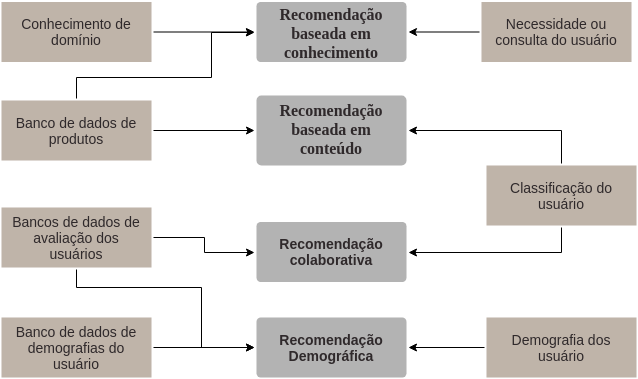
\includegraphics[width=.8\textwidth]{figuras/secao-referencial/tecnicasRecomendacao.png}
\caption{Técnicas de Recomendação e fontes de conhecimento. Adaptado de \cite{burke2007hybrid}.}
\label{img:recomendacao}
\end{figure}



\section{Considerações Finais do Capítulo}

Há indícios de que o perfil do testador possua interferência nas atividades de teste. Os testes realizados acerca dos serviços que chegam ao ITRAC fazem parte de um contexto propenso a se realizar estudos que envolvem os temas abordados neste capítulo de Referencial Teórico.

A partir do conteúdo obtido com a pesquisa bibliográfica especificada em \ref{ch:metodologia} e apresentado neste capítulo, este trabalho busca aplicar conceitos relacionados a perfis de testadores, utilizando de técnicas de trabalhos já publicados sobre sistemas de recomendação, a fim de realizar uma adaptação para consolidação da abordagem discutida no Capítulo~\ref{ch:proposta}. 

% \del{Verifique o parágrafo acima}